\documentclass{beamer}
\usepackage{presentation}

\begin{document}

\frame{\titlepage}

\begin{frame}
  \frametitle{Introduction}
  \begin{quote}{}
    Single Purpose Cloud Connected Tablet for organizing scheduled items by necessity, urgency and frequency
  \end{quote}

  \begin{minipage}{0.33\textwidth}
    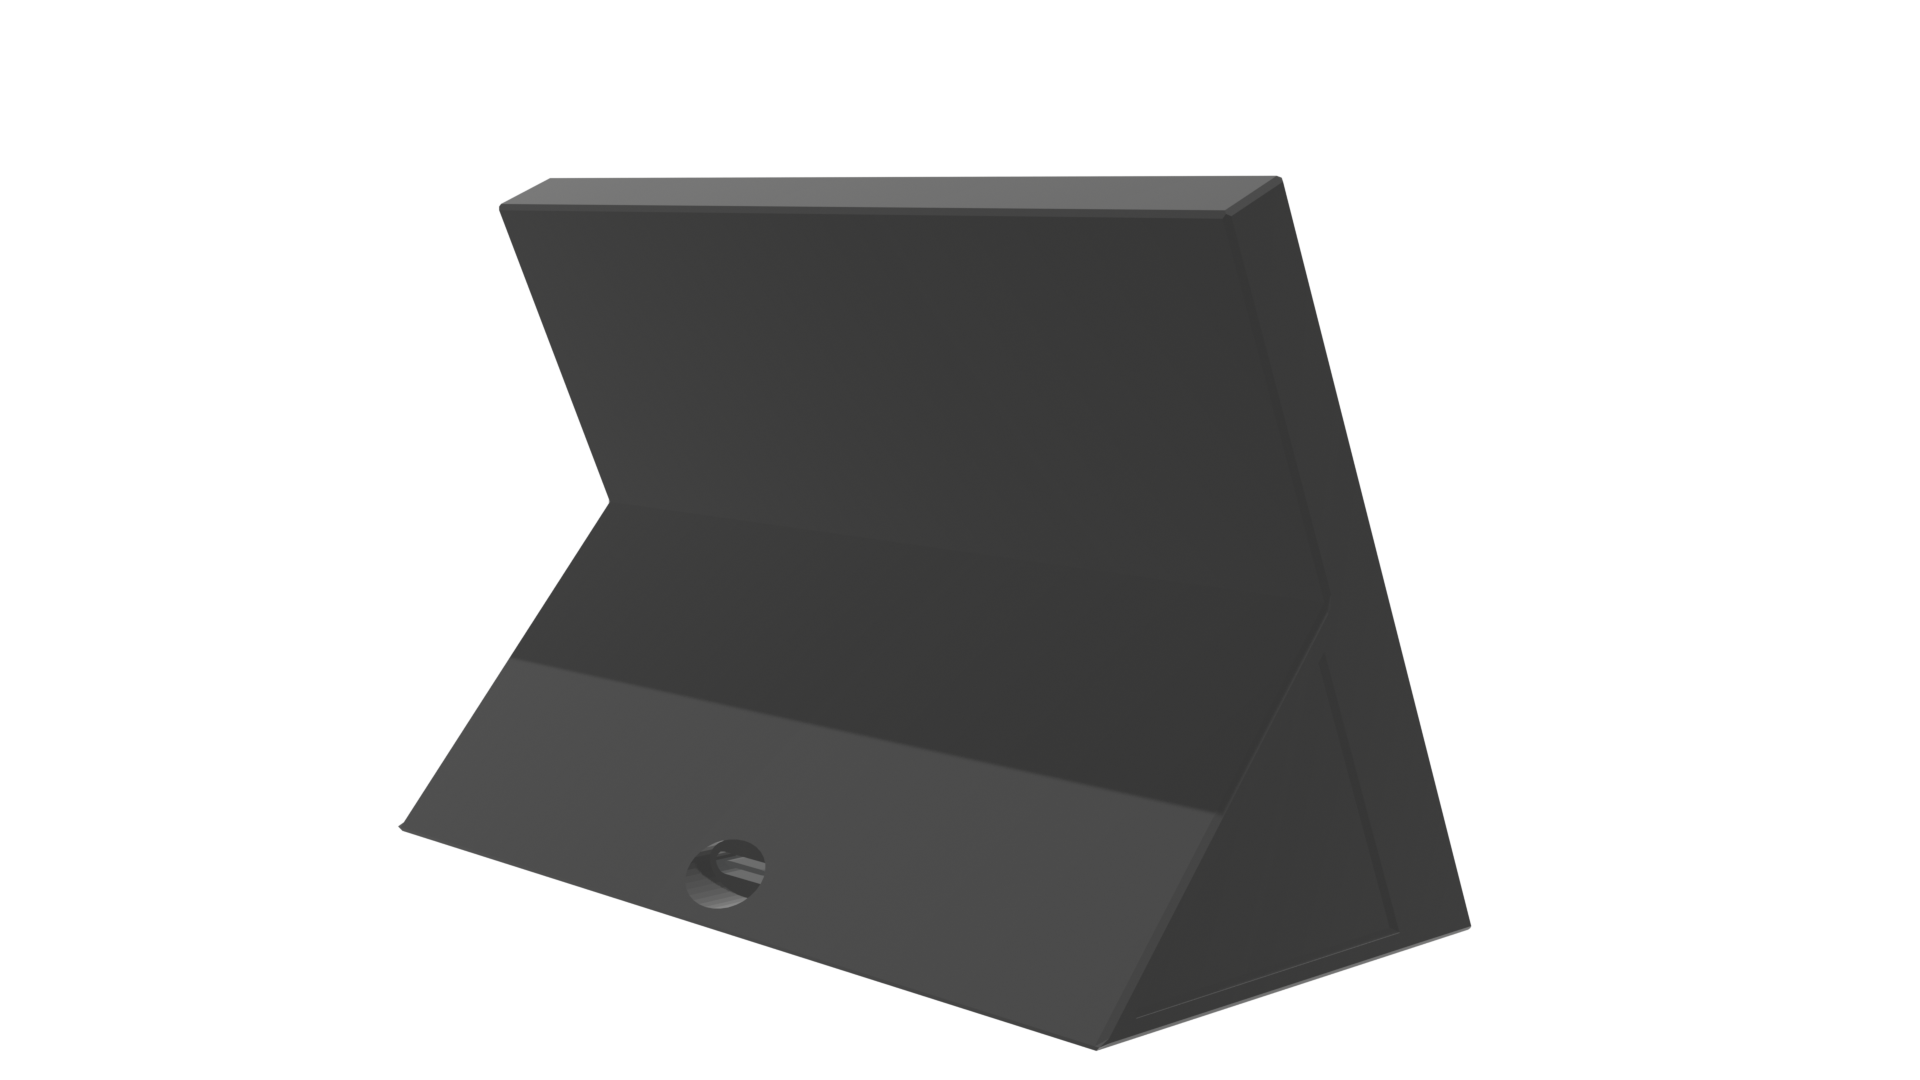
\includegraphics[width=\textwidth]{schedule_companion_render_back.png}
  \end{minipage}
  \hfill
  \begin{minipage}{0.65\textwidth}
    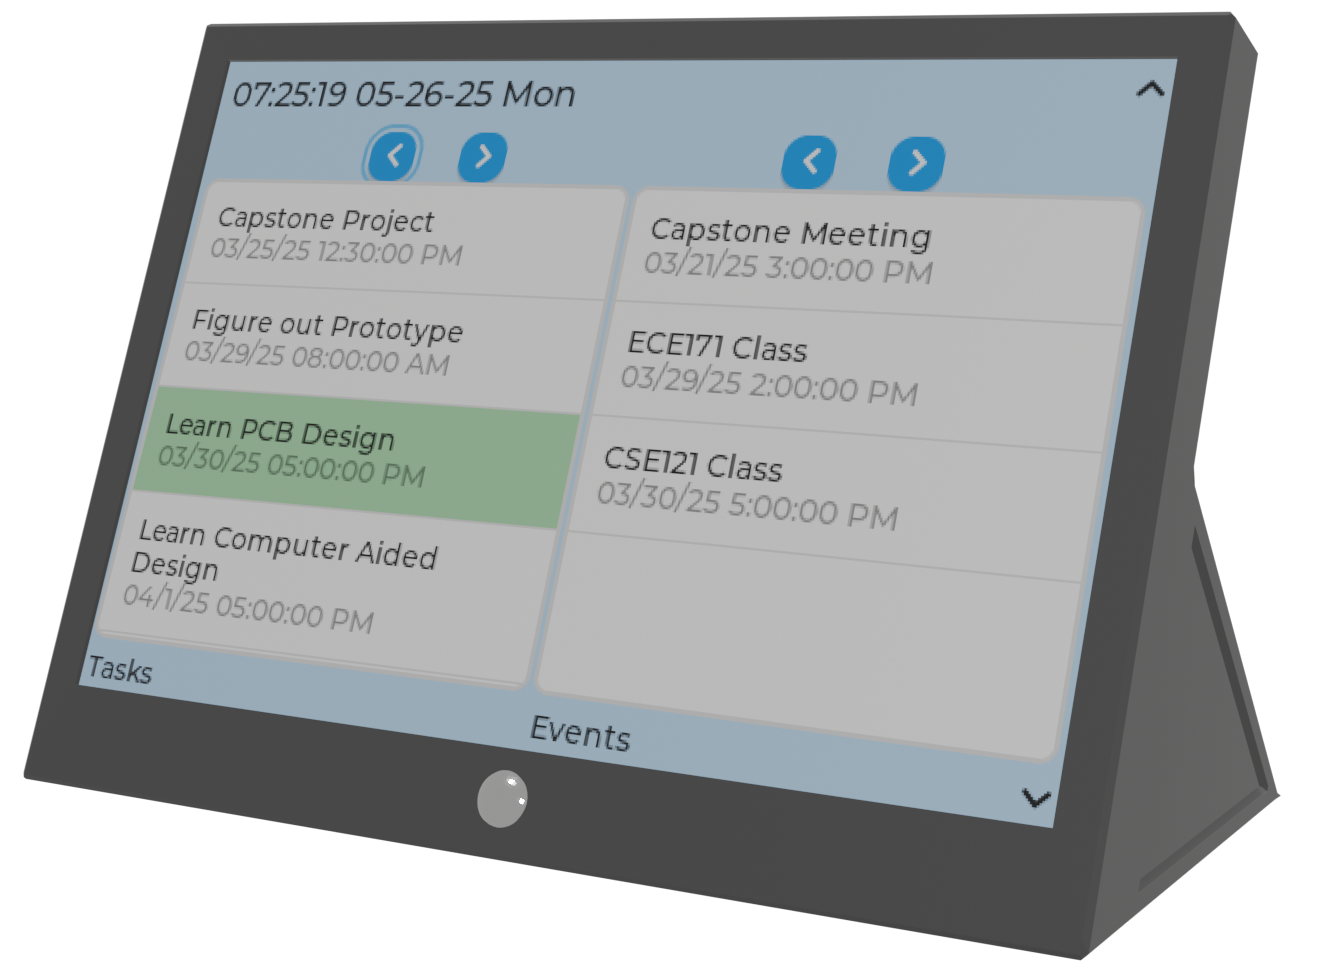
\includegraphics[width=\textwidth]{schedule_companion_render.png}
  \end{minipage}%
  \note[item]{maybe elaborate more on exactly why we did this project}
  \note[item]{The triangular volume on the back of the device serves as a kickstand and case for electronics.}
  \note[item]{Keeps center of gravity low makes it difficult to tip over}
  \note[item]{A large space is necessary to fit two 18650 battery cells which we selected over a specific pouch battery for repairability}
  \note[item]{Provides room for easily assembly and disassembly, good for repairability.}
\end{frame}

\begin{frame}
  \frametitle{Scheduled Activity Design}

  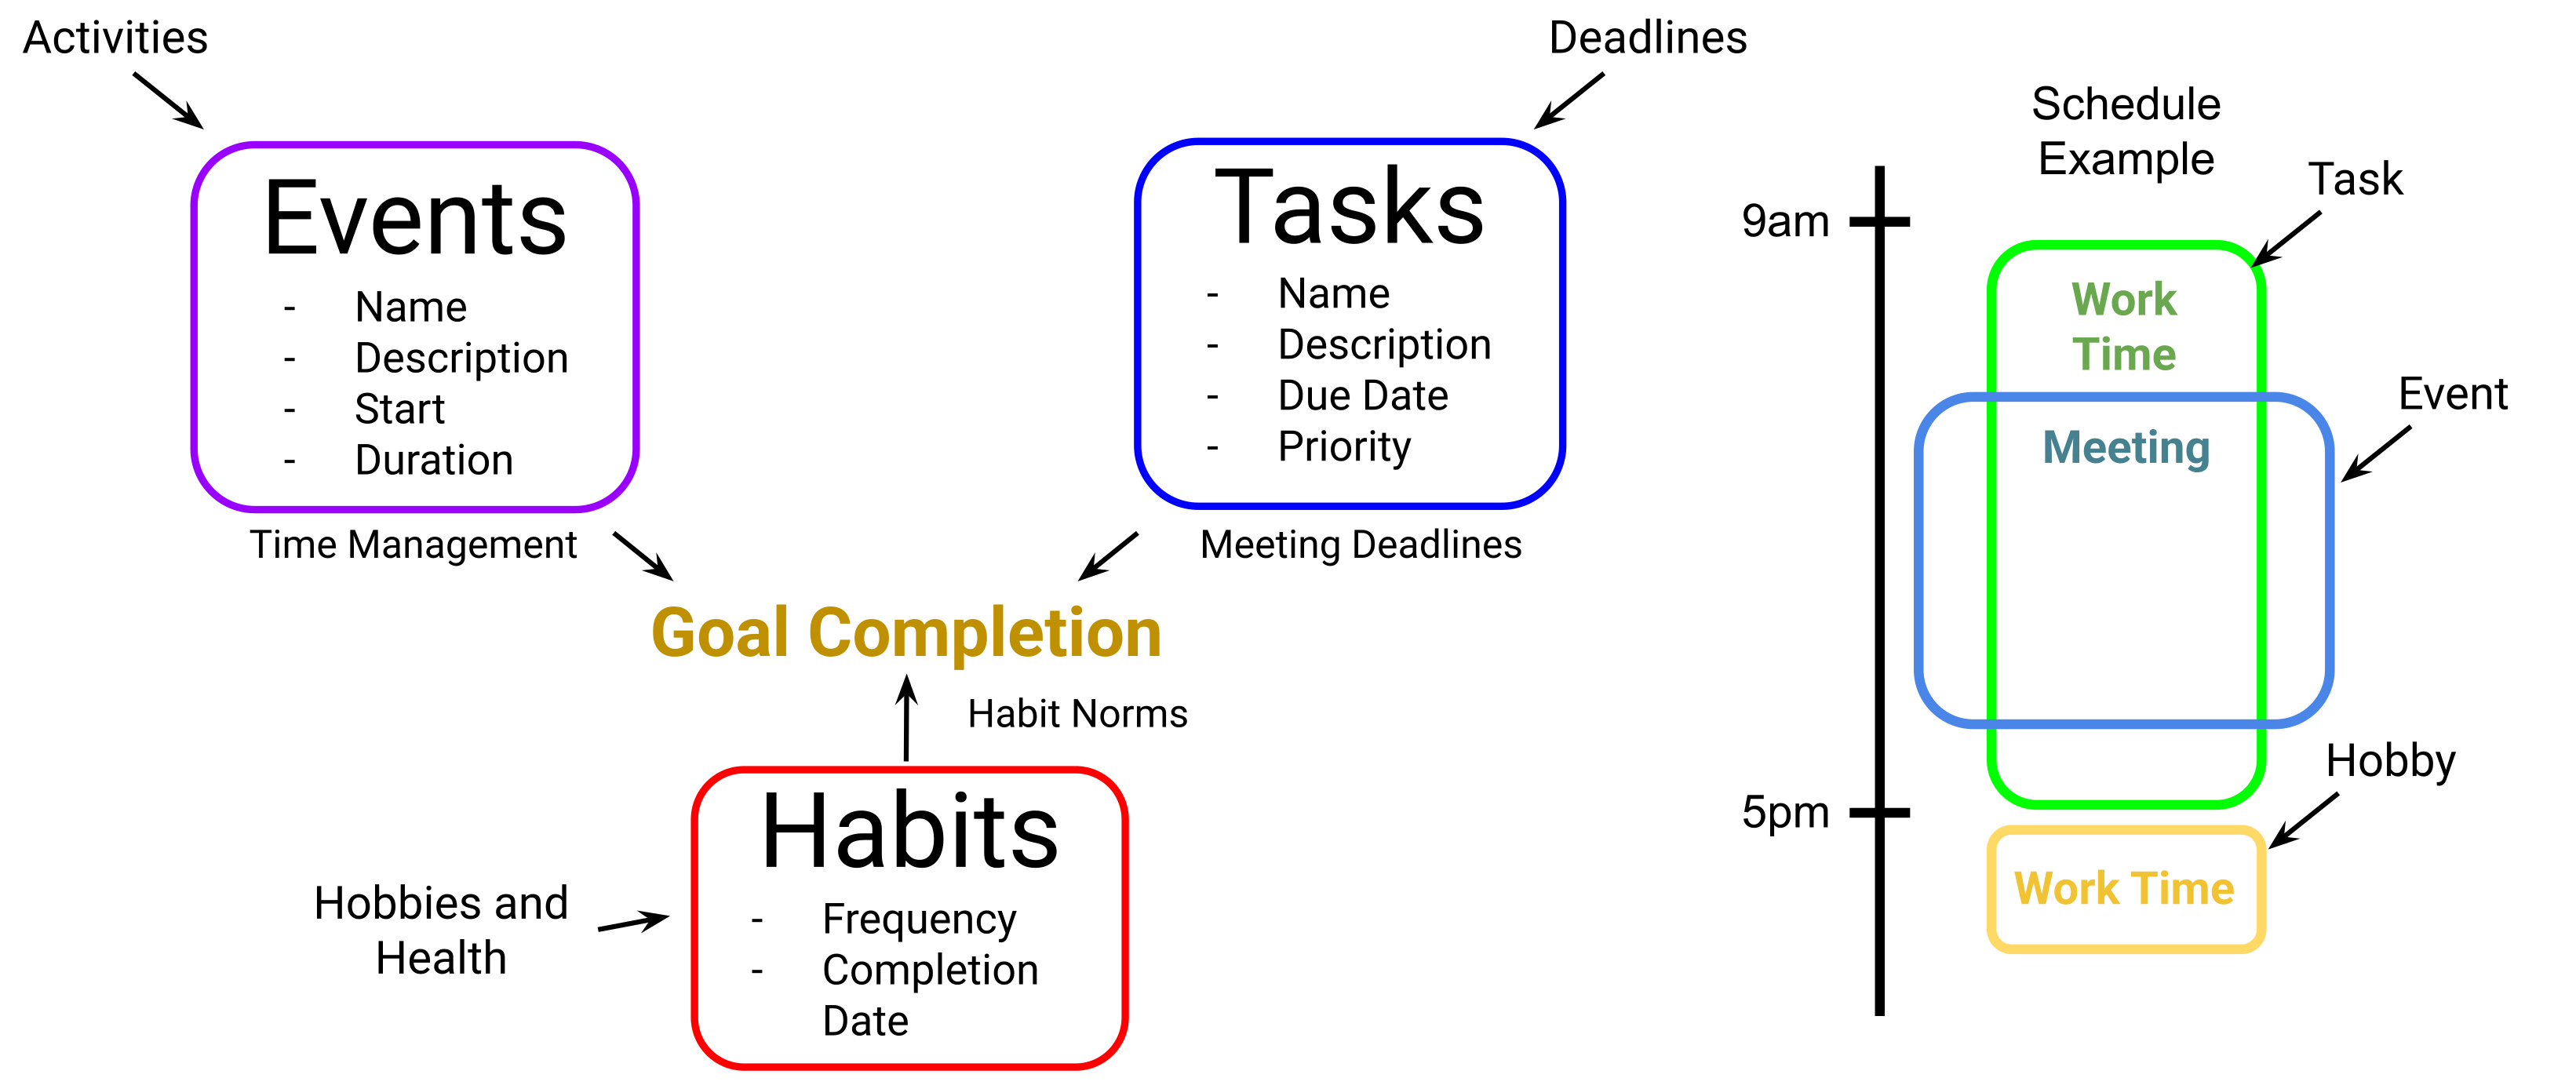
\includegraphics[width=\textwidth]{goal_completion.png}

  \note[item]{The intent of this project is to facilitate \textit{Goal Completion}, which our task managed through \textit{entry management}}
  \note[item]{Tasks are defined objectives that must be completed by a given deadline.}
  \note[item]{Events represent fixed intervals of time and are recorded within the device’s internal calendar.}
  \note[item]{Habits, in contrast to tasks, represent repeated behaviors the user wishes to cultivate.}
\end{frame}

\begin{frame}
  \frametitle{Features}
  \begin{table}
    \centering
    \small
    \begin{tabular}{|p{0.2\textwidth}|p{0.2\textwidth}|p{0.2\textwidth}|p{0.2\textwidth}|}
      \hline
      \cellcolor[HTML]{CFE2F3}Interactive UI           & \cellcolor[HTML]{CFE2F3}Web app                       & \cellcolor[HTML]{CFE2F3}Cloud server               & \cellcolor[HTML]{CFE2F3}Account creation         \\ \hline
      \cellcolor[HTML]{CFE2F3}User / device creation   & \cellcolor[HTML]{CFE2F3}Device management             & \cellcolor[HTML]{CFE2F3}Many devices to one user   & \cellcolor[HTML]{CFE2F3}Many users to one device \\ \hline
      \cellcolor[HTML]{CFE2F3}Focus Mode               & \cellcolor[HTML]{CFE2F3}Task and event implementation & \cellcolor[HTML]{CFE2F3}Habits implementation      & \cellcolor[HTML]{CFE2F3}Offline usage            \\ \hline
      \cellcolor[HTML]{CFE2F3}Wi-Fi provisioning       & \cellcolor[HTML]{CFE2F3}Real-time clock display       & \cellcolor[HTML]{CFE2F3}Encrypted data in transit  & Battery powered                                  \\ \hline
      Configurable user settings                       & Phone app                                             & Touch controls                                     & Haptics and audio feedback                       \\ \hline
      Schedule sorting                                 & Time blocking                                         & Power button                                       & Chassis                                       \\ \hline
    \end{tabular}
  \end{table}

  \renewcommand{\thefootnote}{\roman{footnote}}
  \footnotetext[0]{Successfully prototyped features are highlighted}
\end{frame}

\begin{frame}
    
  \frametitle{What did we learn from the prototype?}

  \begin{columns}
    \column{0.5\textwidth}
    What worked:
    \begin{itemize}
      \item SQLite3
      \item Persistence
      \item Web server
      \item SoftAP Wi-Fi provisioning
    \end{itemize}

    \column{0.5\textwidth}
    What is improved and included in the manufactured product:
    \begin{itemize}
      \item Comunication protocol
      \item SoC specs
      \item Device authentication
      \item Additional software features
      \item Screen size and touch
      \item Haptics and audio 
      \item Bluetooth Wi-Fi provisioning
    \end{itemize}
  \end{columns}
  
  \note[item]{LVGL already custom external gpu rendering}
  
  \note[item]{no stores messages $\rightarrow$ need to send entire backup every time}
  \note[item]{An HTTP server that responds to "changes since X" is a more efficient approach.}
  \note[item]{Ideal gets whole backup on power on, gets new messages as it polls}

  \note[item]{ESP32-C3: RISC-V SoCs do not support memory expansion}
  \note[item]{Discuss potential alternatives: ESP32-S3, Teensy 4.1, STM32H7 line, Pi Zero 2W}
  \note[item]{Components: add haptics, audio, improve screen and touch}
  \note[item]{Additional features: time blocks, custom schedule organization}
  \note[item]{BLE Wi-Fi provisioning component already exists}

\end{frame}

\begin{frame}
  \frametitle{Server Architecture}

  \begin{center}
    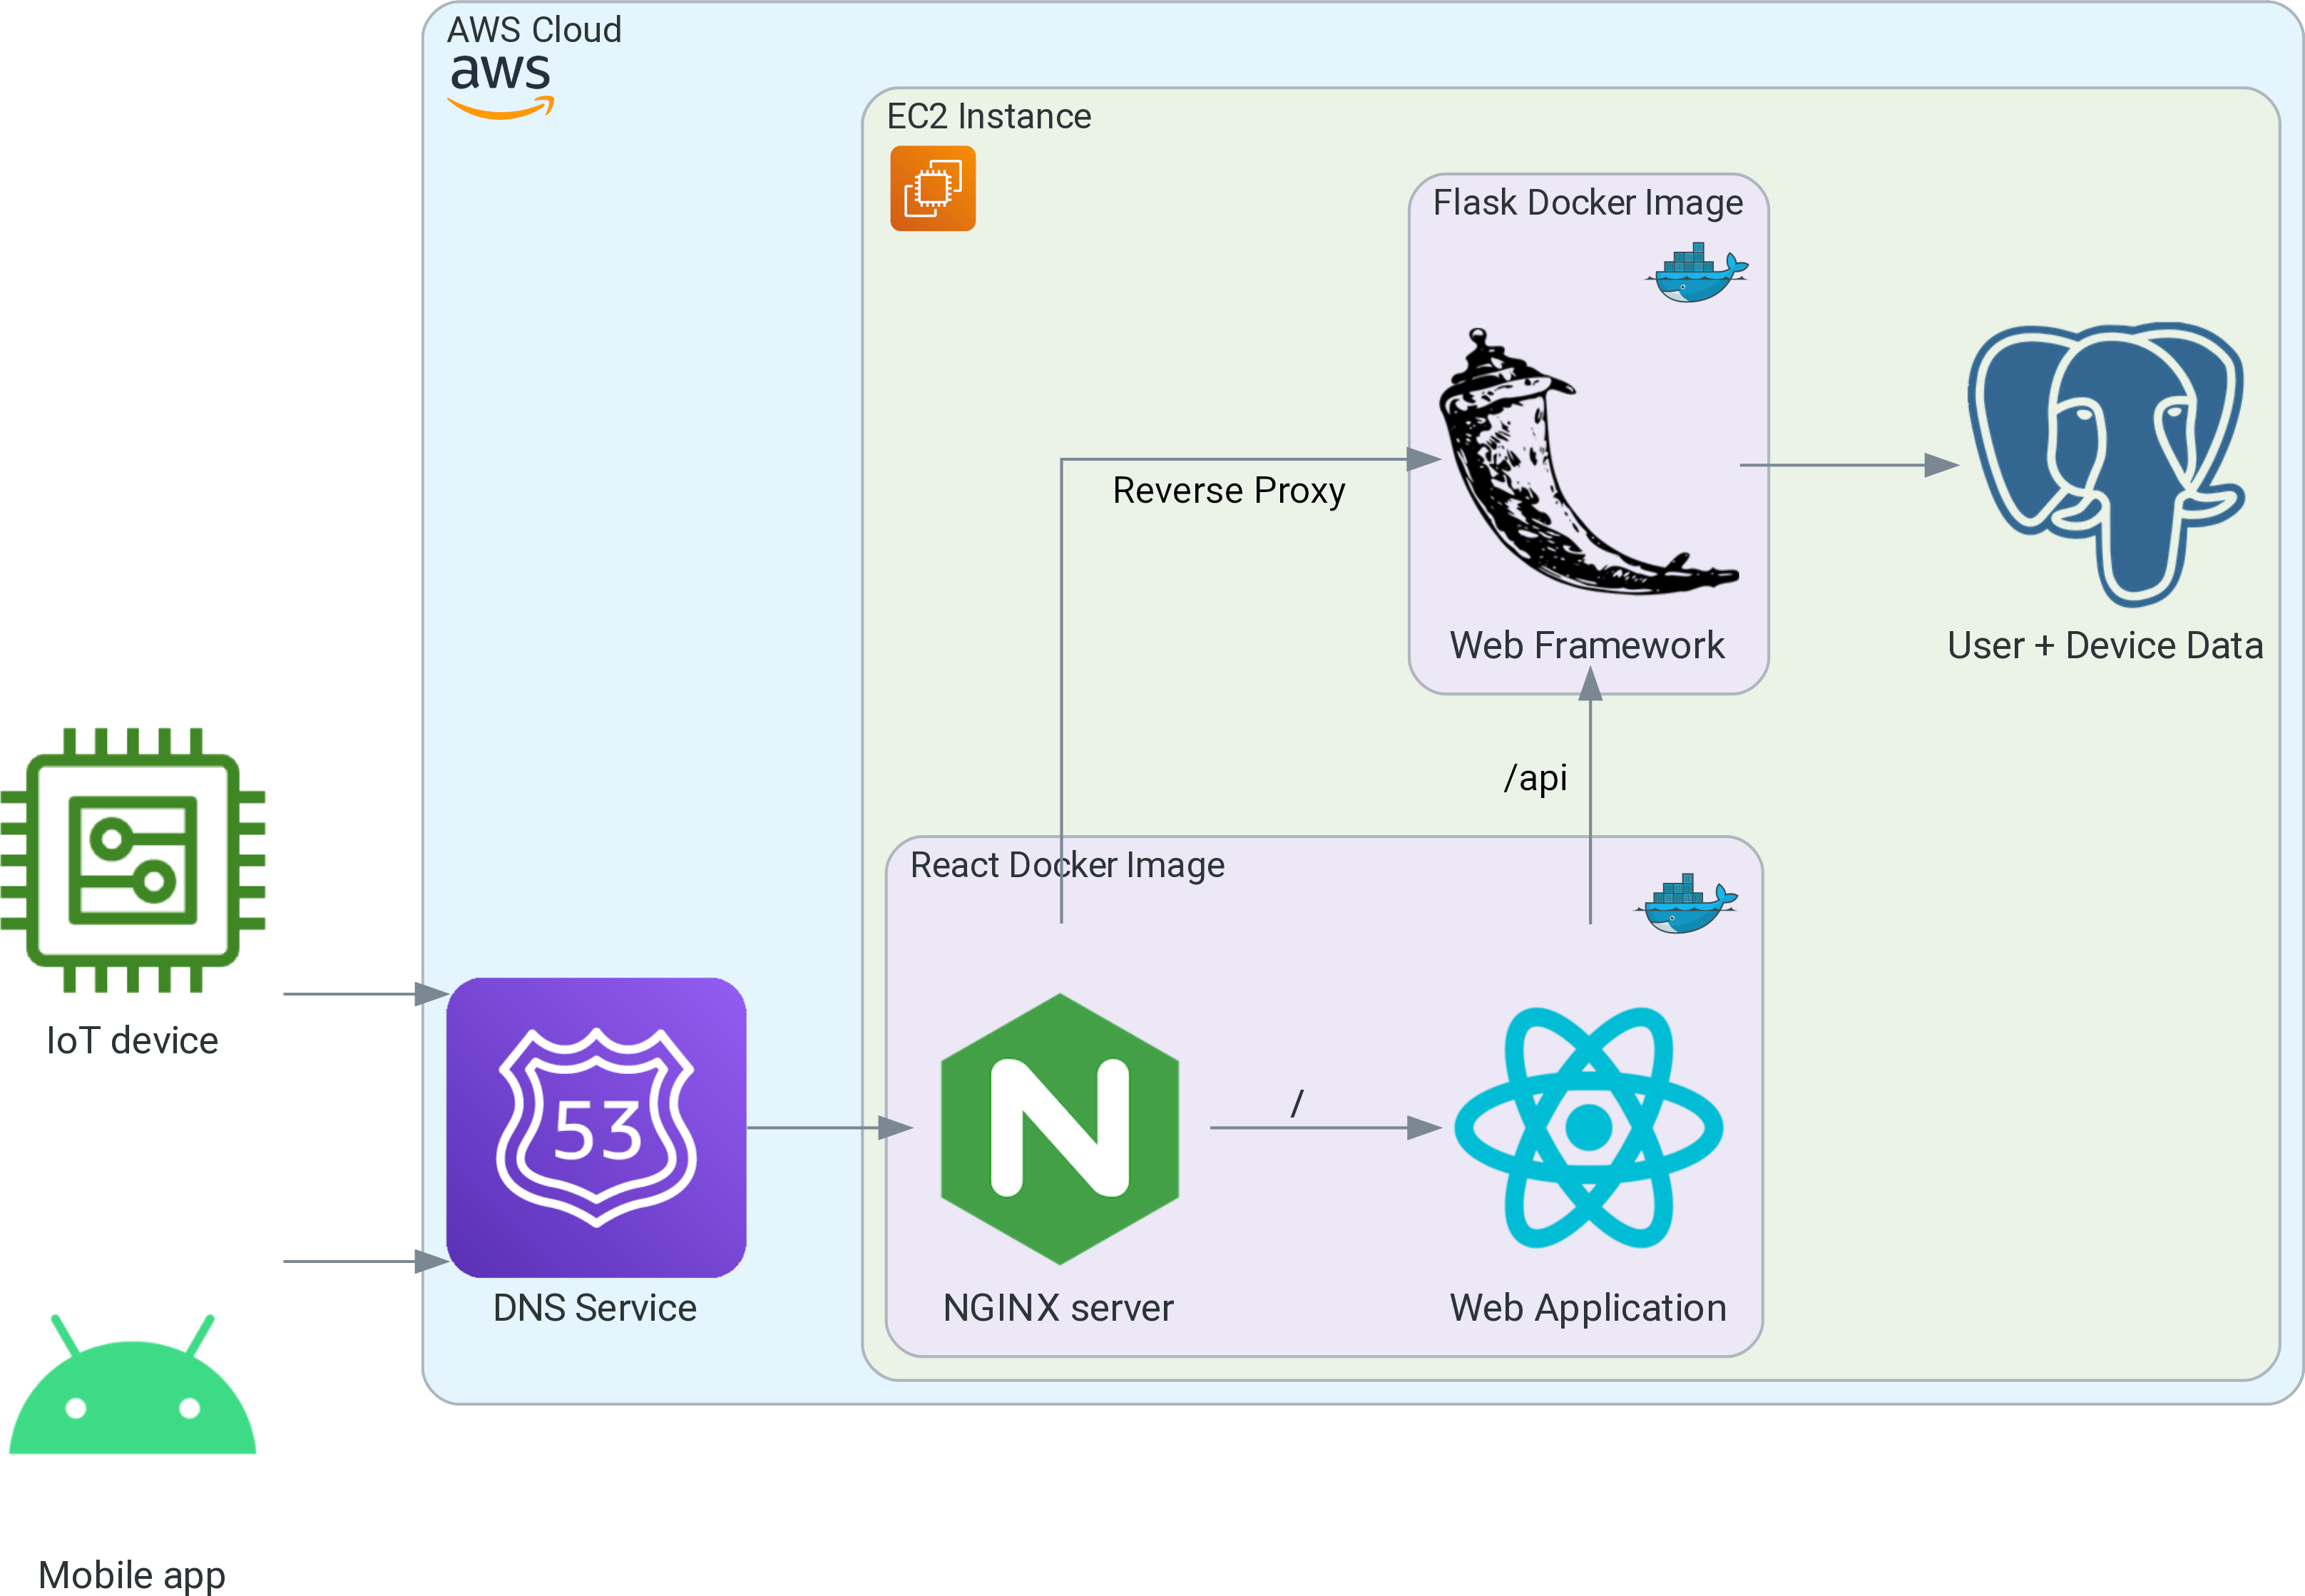
\includegraphics[width = 0.9 \textwidth]{data_flow.png}
  \end{center}

  \note[item]{React web app and the device will make requests to "/api" to
  interact with the server data}
  \note[item]{Both user and device will interact with the api after ensuring
  they have an un-expired jwt}
  \note[item]{With device jwt, we will have better security and a proper
  device authentication process}

\end{frame}
\begin{frame}
  \frametitle{Wiring Diagram}
  \begin{center}
    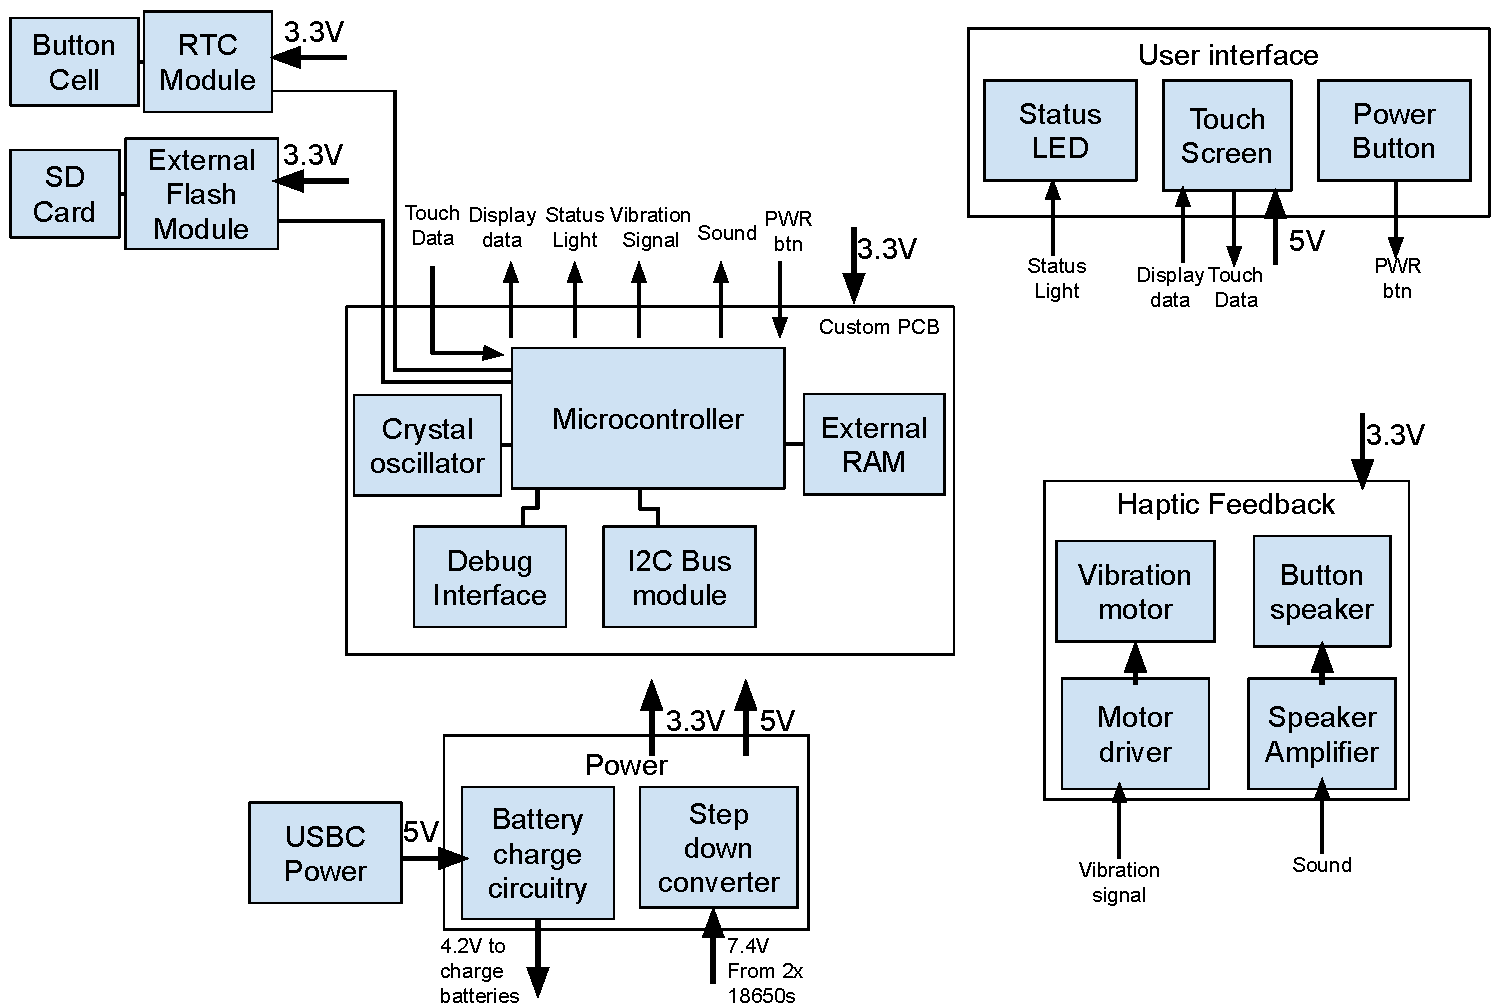
\includegraphics[width = \textwidth]{product_pcb_diagram.pdf}
  \end{center}
  \note[item]{made abstract for different potential components}
\end{frame}

\begin{frame}
  \frametitle{Tests}
  \begin{columns}
    \column{0.5\textwidth}
    Prototype feasible tests:
    \begin{itemize}
      \item Wifi Provisioning
      \item Boot time 
      \item Sync time 
      \item New User Registration 
      \item New Device Addition
      \item Many to One Support 
      \item Data Persistence
    \end{itemize}

    \column{0.5\textwidth}
    Manufactured product tests:
    \begin{itemize}
      \item Durability
      \item Thermal
      \item Battery life cycle
      \item Haptics and sound
    \end{itemize}
  \end{columns}
  \note[item]{Durability testing: includes chemical testing, drop testing, tensile testing, UV testing}
  \note[item]{Battery life cycle: charge speed, battery degradation, battery life}
\end{frame}

\begin{frame}
  \frametitle{Test Results}
    \centering
    \begin{tabular}{l
    >{\columncolor[HTML]{9AFF99}}l }
    \hline
    Test                  & \cellcolor[HTML]{FFFFFF}Results \\
    \hline
    Wifi Provisioning     & PASS                         \\
    Boot time             & PASS                         \\
    Sync time             & \cellcolor[HTML]{FFCCC9}FAIL \\
    New User Registration & PASS                         \\
    New Device Addition   & PASS                         \\
    Many to One Support   & PASS                         \\
    Data Persistence      & PASS                         \\
    \hline
    \end{tabular}
\end{frame}

\begin{frame}
  \frametitle{Specs}
  \begin{table}
    \centering
    \begin{tabular}{lllll}
      \hline
      Specifications                & Units   & \multicolumn{3}{l}{Value} \\
      \hline
      Price                & USD     & \$100     & $\rightarrow$ & \$150 \\
      Devices per user     & Devices & Unlimited & $\rightarrow$ & 10    \\
      Users per device     & Users   & Unlimited & $\rightarrow$ & 10    \\
      Cloud sync time      & Seconds & 10        & $\rightarrow$ & 100m  \\
      \# entries           & Entries & 100       & $\rightarrow$ & 8000  \\
      Database Size        & Bytes   & 60G       & $\rightarrow$ & 32M   \\
      Standby Battery life & Hours   & 200       & $\rightarrow$ & 168    \\
      Wakeup time          & Seconds & 3         & $\rightarrow$ & 100m  \\
      \hline
    \end{tabular}
  \end{table}
\end{frame}

\begin{frame}
  \frametitle{Questions?}
    \centering
    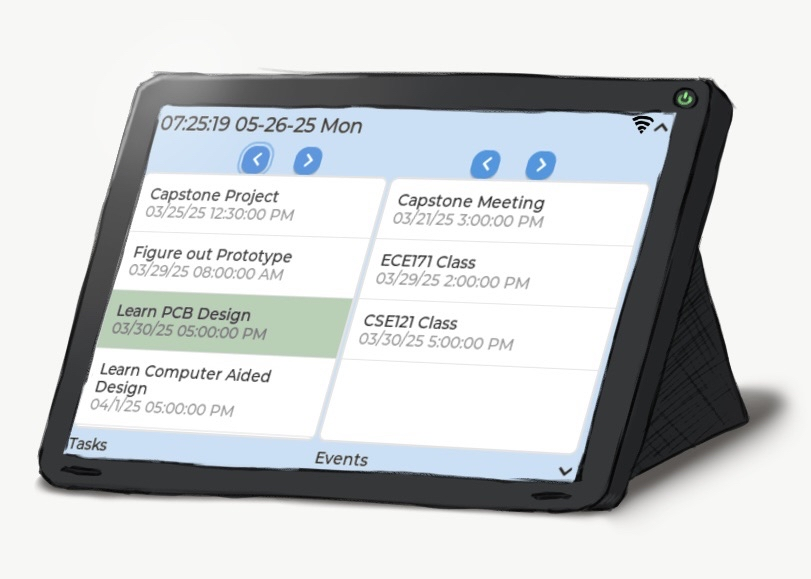
\includegraphics[width = 0.7\textwidth]{aestheticRender.png}
\end{frame}
\end{document}
